\documentclass[a4paper,12pt]{journal}
\usepackage[dvipsnames, svgnames, x11names]{xcolor} 
\usepackage{amsmath}
\usepackage{amssymb}
\usepackage[margin=2.5cm]{geometry}
\usepackage{graphics}
\usepackage{ulem}
\usepackage{setspace}
\usepackage{listings}
\usepackage{algorithm}  
\usepackage{algpseudocode}  
\usepackage{amsmath}  
\usepackage{xcolor}
\usepackage[greek,english]{babel}
\usepackage{chemformula}
\usepackage{wrapfig}
\usepackage{multirow}
\usepackage{booktabs}
\usepackage{fancyhdr}
\usepackage{pgfplots}
\usepackage{tikz}
\pagestyle{fancy}
\rmfamily
\fancyhf{}
\fancyfoot[R]{\thepage}
\fancyhead[R]{VE475 HW1}
\title{VE475 Homework 1}
\author{Anna Li \\Student ID: 518370910048}
\date{\today}
\lstset{
	columns=fixed,     
	numbers=left,                                        % 在左侧显示行号
	numberstyle=\tiny\color{gray},                       % 设定行号格式
	frame=none,                                          % 不显示背景边框
	backgroundcolor=\color[RGB]{245,245,244},            % 设定背景颜色
	keywordstyle=\color[RGB]{40,40,255},                 % 设定关键字颜色
	numberstyle=\footnotesize\color{darkgray},           
	commentstyle=\it\color[RGB]{0,96,96},                % 设置代码注释的格式
	stringstyle=\ttfamily\slshape\color[RGB]{128,0,0},   % 设置字符串格式
	showstringspaces=false,                              % 不显示字符串中的空格                                        % 设置语言
}
\begin{document}
	\maketitle
	\section*{Problem 1}
	\subsection*{1.}
	We try every situations for the ciphertext "EVIRE", and get the 25 situations  by switching K from 0 to 25, and find that there are two possibilities: river when K = 13 and arena when K = 4\\
	\subsection*{2.}
	First, we could convert dont and ELNI into $2\times 2$, which is:
	\begin{equation}
		dont=\begin{pmatrix}
			3&14\\13&19\\
		\end{pmatrix}\quad 
	ELNI = \begin{pmatrix}
		4&11\\13&8\\
	\end{pmatrix}\quad 
	\end{equation}
suppose the encryption matrix is K, we can get:
\begin{equation}
K=dont^{-1}\cdot ELNI \mod 26
\end{equation}
\begin{equation}
dont^{-1}=\frac{1}{125}\begin{pmatrix}-19&14\\13&-3\\\end{pmatrix}\mod 26 = \begin{pmatrix}
	-95&70\\65&-15\\
\end{pmatrix}
\end{equation}
\begin{equation}
K=\begin{pmatrix}
10&9\\13&23\\
\end{pmatrix}
\end{equation}
\subsection*{3.}
since $n|ab$, we could deduce that 
$$\exists r\in\mathbb{R}, nr=ab$$
since $gcd(a,n)=1$, we could deduce that
$$\exists s,t\in\mathbb{R},as+nt=1$$
Therefore
$$b=b(as+nt)=nrs+bnt=n(rs+bt)$$
Therefore, $n|b$
\subsection*{4. }
\begin{equation}
\begin{array}{r c l}
30030&=&257\times 116+218\\
257&=&218\times 1+39\\
218&=&39\times5+ 23\\
39&=&23\times 1+16\\
23&=&16\times 1 +7\\
16&=&7\times 1+9\\
7&=&9\times 0+7\\
9&=&7\times 1+2\\
7&=&2\times 3+1\\
2&=&1\times 2+0\\
\end{array}
\end{equation}
Therefore, gcd(30030,257)=1\\
since $\sqrt{257}\in(16,17)$, we could check 2,3,5,7,11,13\\
since
$$gcd(257,2)=1\quad gcd(257,3)=1\quad gcd(257,5)=1$$
$$ gcd(257,7)=1\quad gcd(257,11)=1\quad gcd(257,13)=1$$
Therefore, 257 is a prime number
\subsection*{5.}
if the attacker get the ciphertext and part of the plaintext, they will solve out the key soon. Therefore, when the next time the one time pad use the same key, the attacker could easily solve the whole plaintext. Therefore, this is dangerous.
\subsection*{6. }
Since secure means that the attacker has to compute at least $2^128$ operations to break the encryption it suffices to calculate.
$$\sqrt{n\log n}=128\Rightarrow n=4487$$
Therefore, at least 4487 size of graph should be used
\section*{Problem 2}
\subsection*{1.}
Vigenere Cipher is a method of encryption, which is similar to ceaser cipher but is more secure than it. In the Vigenere cipher, we first choose a keyword with n length, and then repeat it. This keyword means that how many steps should the letter shift in each position. \\
And we could look up this table to encrypt the plain text:
\begin{figure}[ht]
\centering
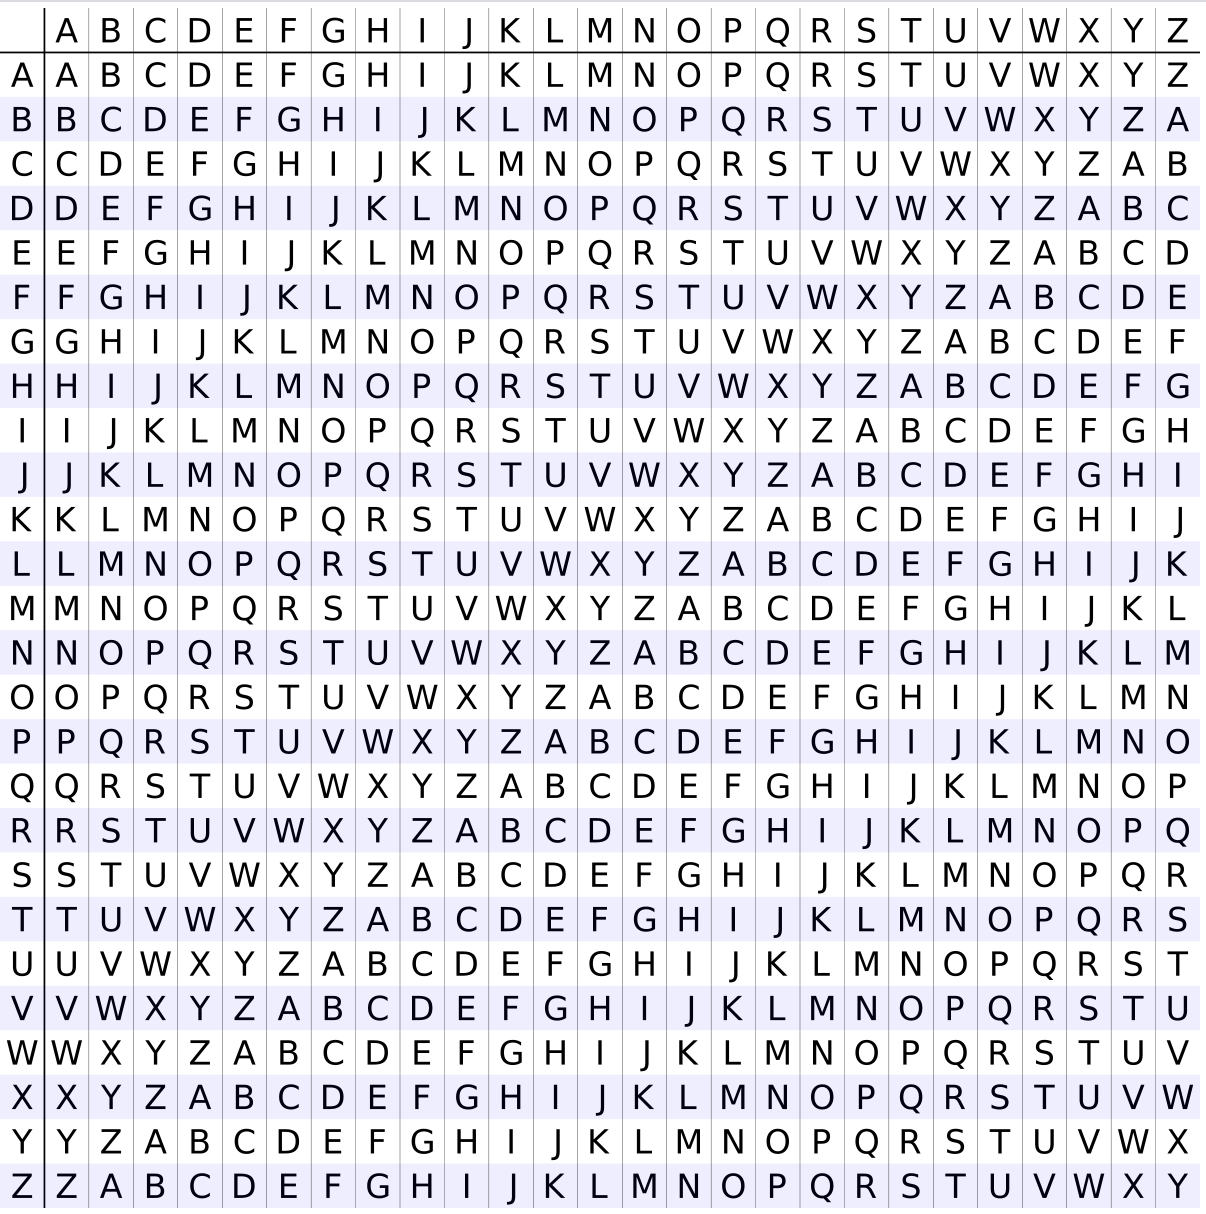
\includegraphics[scale=0.5]{1.png}
\caption{Table of Vigenere cipher}
\end{figure}
\subsection*{2. }
\subsubsection*{a)}
Because the cipher text repeats the same six letters several hundred times, and the relative position difference between the cipher text is the same as the difference between the key. Therefore, Eve can suspect that the plain text is one repeated letter.
\subsubsection*{b)}
Since the cipher text always repeat with period of 6, Eve can guess the key length
\subsubsection*{c)}
Eve could shift this repeated six letters from 0 to 25, and find out the only one possibility, since no English word of length six is a shift of another English word.
\end{document}
